\chapter{Implementing a MQTT Server}
\label{intro} 


\abstract{
My part of the project is to provide a stable and fast communication interface.
One of the challenges is to find a free service that provides an MQTT interface. It is also my job to provide the code for establishing a connection.
The result is a free MQTT server in the solace cloud. The code to connect has also been successfully completed.
}

\section{Introduction}
\label{sec:1}


Connected systems can be found almost everywhere. The refrigerator speaks to the dishwasher. The bell no longer rings but sends a message to your smartphone. Other examples can be observed both at home and in the entire environment.

The key to success in such applications is information transfer. The embedded systems must be able to exchange information. Every embedded system must understand each other and also be able to interpret the data. The next logical step is to connect the individual components of a city. This chapter explains exactly how communication takes place in this fictional city.

This chapter deals with data transfer with MQTT between several end devices. The end devices can only be reached via the Internet, not via the local network.


\section{Related works}
\label{sec:2}
The paper \cite{inbook} describes a work similar to that described here. The paper is also about a smart city, but it is not designed to connect public facilities, but rather was set up as an example with just a few sensors. The central component, the communication, is however similar. In this case, data from the vehicle is published and used by the facilities to guarantee, among other things, the best possible health care.

\section{Concept}
\label{sec:3}
The project is about a smart city Network. This means, that every entity of the City is connected to every other entity. When a car crashes, the police, firefighters and ambulances get informed. Part of the information is the hardness of the accident. What exactly did happen when and where? This was just one example of all the possible applications. My part in this project ist to get the messages from the sender to the listener.
\newline

%\\ requirements table
\begin{tabular}[h]{ll}
\vspace{10}
Request number & Name \\
FREQ00 & The interfaces between the participants must be documented.\\
FREQ01 & The broker must be accessible via the internet.\\
FREQ02 & The broker must be maintainable via a web interface.\\
FREQ03 & Communication must take place via the defined topics.\\
FREQ04 & End devices must be able to log on to the server.\\
FREQ05 & End devices must be able to tell the server which topics they want to subscribe to.\\
FREQ06 & The broker must receive information.\\
FREQ07 & The broker must forward information as needed.\\

NFREQ00 & Communication must take place via a protocol.\\
\vspace{10}
\end{tabular}
Because of this requirements and dependencys to the parts of this project we choosed Mqtt. Mqtt (Message Queuing Telemetry Transport) is a protocol that manages the communication inside of decentralized embedded systems. It is lightweight and can be used in most of the embedded languages as a library. 
%\\What excactly is MQTT?
%\\MQTT is the short term for "Message Queuing Telemetry Transport". This is a network based communication protocol for machine to machine communication. It is a lightweight protocol that transport messages with low bandwith usage.

The central point in the network is the broker. Among other things, this saves the endpoints and how they can be reached. The broker also saves which end point sends which messages in the topic.

The broker can either run in the local network or in the cloud. However, if the broker is running in the cloud, there is a single point of failure. This can be done by either multiple brokers that perform load balancing.

In order to have a backup, a local broker can cache the incoming messages and forward them to the cloud broker when the cloud broker is available again.

The broker only offers the functionality to forward the messages. By default, the messages are not saved. If it is expected that a client temporarily loses the connection to the broker, a persistent connection can be reserved. This means that the broker caches all missed messages. These are then all made available to the client the next time the connection is established.

Communication is based on so-called topics. These topics act as a channel in which any text-based message can be sent.

Endpoints can subscribe to these topics. If you have subscribed to the topic, each message will be forwarded to the endpoints.

The programming language python was selected based on previous projects in this language that led to basic knowledge. Another reason was the simplicity and usability on different systems.

The function of the broker can be seen in Figure \ref{mqttFunktion} The vehicle can be seen on the left. This publishes your own speed. The broker in the middle forwards this information both to the mobile device and to the backend. In this project there is no need to forward the information to a mobile device. The backend is explained in more detail in the following chapter.
\begin{figure}
\sidecaption
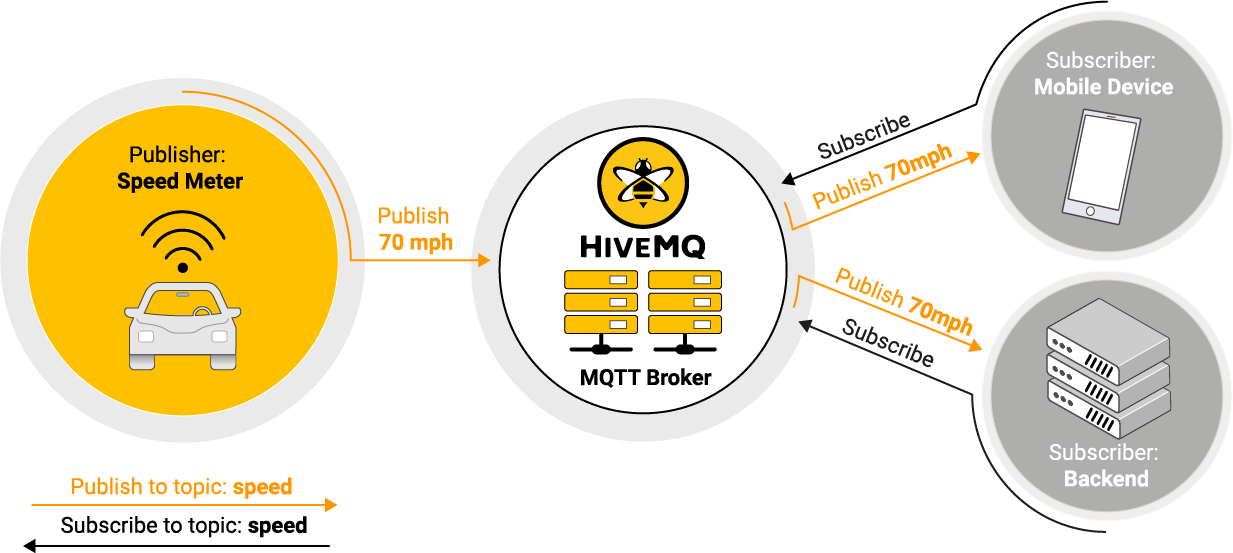
\includegraphics[scale=.25]{chapters/chapter1_dominic/mqtt.png}
\caption{this is a picture}
\label{mqttFunktion}
\end{figure}

\section{Implementation}
\label{sec:4}
This chapter describes how to connect to a cloud-based MQTT server. Furthermore, the sending and receiving of messages is described in so-called topics. This is underpinned as an example with code snippets.
%   if you have class diagram
%\\ or an image that show parts of your system
%\\ screenshots of part of your code
\subsection{Establishing the connection}
As noted in chapter \ref{sec:3} the paho.mqtt library is used. Figure \ref{imports} shows the import of the paho.mqtt library into the python program.
The second import is the library time. This supports sleep cycles and repetitions after a given time.
\begin{figure}
\sidecaption
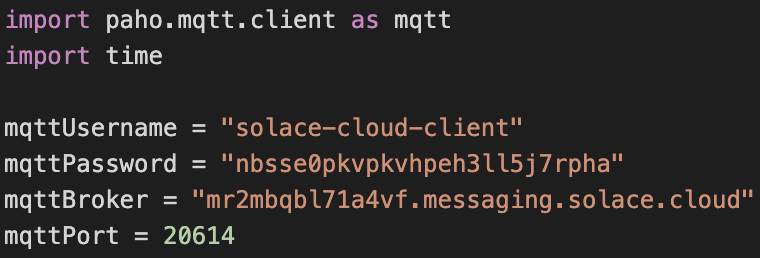
\includegraphics[scale=1]{chapters/chapter1_dominic/Imports.png}
\caption{this is a picture}
\label{imports}
\end{figure}
Lines 3 to 7 list the parameters for establishing the transmission. the username and password are the access controls to the network. These were generated automatically and provided by the Cloud mqtt server. The MQTT broker and port is the central point to which these messages are sent.

In figure \ref{connection} you can see the code with which the connection to the broker is established.
The mqtt.client object is created in line one. The on connect event is added in the second line (see figure \ref{onConnect}). The specific access data are assigned to the client object in lines 3 and 4. This is the data as shown in Figure \ref{imports}.
\begin{figure}
\sidecaption
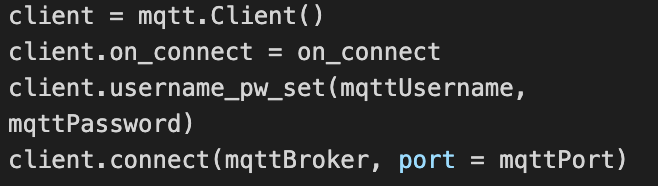
\includegraphics[scale=1]{chapters/chapter1_dominic/establishConnection.png}
\caption{this is a picture}
\label{connection}
\end{figure}
\begin{figure}
\sidecaption
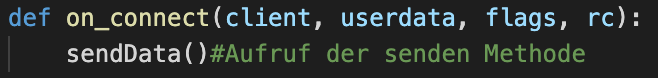
\includegraphics[scale=1]{chapters/chapter1_dominic/onConnect.png}
\caption{this is a picture}
\label{onConnect}
\end{figure}

\subsection{Publish}
Image \ref{sendData} shows the code where the data will be send to the broker. In the second line the topic gets initialised with the string "/hshl/test". This test topic is just used to test the clients if they work correctly and can send and receive data.
\begin{figure}
\sidecaption
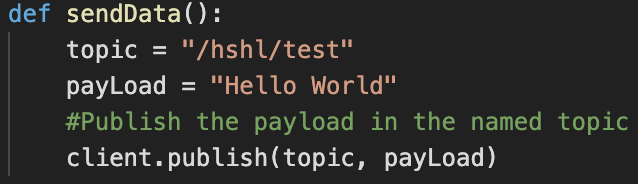
\includegraphics[scale=1]{chapters/chapter1_dominic/sendData.png}
\caption{this is a picture}
\label{sendData}
\end{figure}
%\\ explain the main parts of the code
%\\ make a relation between the functionalities of the system and the requirements
%\\ like: this part of the code does that which is described in the requirement FR1.


\subsection{Receive}

The client must subscribe to the topic so that messages can be received. As soon as a message is sent in the subscribed topic, the event in Figure \ref{onMessage} is called.
With the method shown in figure \ref{onMessage} there are three parameters. The relevant one is the payload. This contains the actual data that should be sent. In the second line, the data is decoded using the UTF-8 character set. For readability, the current time stamp is shown in the following lines in addition to the actual payload.
\begin{figure}
\sidecaption
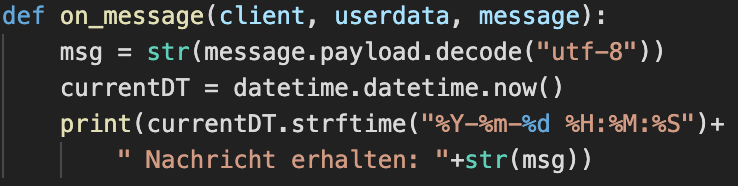
\includegraphics[scale=0.8]{chapters/chapter1_dominic/onMessage.png}
\caption{this is a picture}
\label{onMessage}
\end{figure}


\section{Results}
\label{sec:5}
%   show what is working
% which requirements are not implemented?
% what could you have done in a different way?
In summary, all the requirements mentioned in Chapter \ref{sec:3} were met. The functionality is also guaranteed.

In figure \ref{subber} you can see the output of the subscriber. As can be seen, the connection establishment is accepted by the server. 
\begin{figure}
\sidecaption
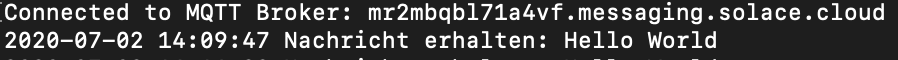
\includegraphics[scale=0.75]{chapters/chapter1_dominic/sub.png}
\caption{this is a picture}
\label{subber}
\end{figure}
The last line of the output shows that a message was received in the topic / hshl / test. The output of the sending can be seen in Figure \ref{pubber} In the first line here as well as when receiving the confirmation that a connection to the Cloud MQTT server has been established.
\begin{figure}
\sidecaption
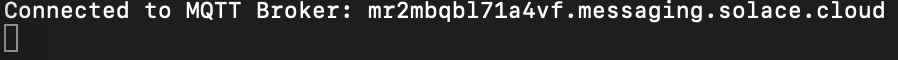
\includegraphics[scale=0.75]{chapters/chapter1_dominic/pub.png}
\caption{this is a picture}
\label{pubber}
\end{figure}

The FREQ00 requirement was met by the MQTT standard.
The broker can be reached via the Internet. This was achieved through the cloud server. This also ensures the requirement of maintainability with a web interface (FREQ02).

The requirement specified in FREQ03 is met by the topic specifications of the professor.

The users need log in to the server. This is done with the user data which are explained in chapter ..

Subscribing to topics is prescribed by the MQTT protocol. This also fulfills requirement FREQ05.



\newpage
\bibliographystyle{IEEEtran}
\bibliography{./chapter.bib}